% vim: set fenc=utf-8 ft=latex encoding=utf-8
% -*- mode: latex; coding: UTF-8; -*-
%!TEX root = knowledge-curation.tex
\section{Results}
\label{cha:findings}

This section presents the findings of our study that answer each research question.

\subsection{RQ-1. \rqa}
\label{cha:findings-types}

From the messages from the Stack Overflow R tag and R-help mailing list,  we identified five main types of knowledge:
\begin{enumerate*}[label=(\arabic*)]
\item Questions,
\item Answers,
\item Updates,
\item Flags, and
\item Comments.
\end{enumerate*}
Each of these types of further divided into sub-types. Table~\ref{table:type-of-knowledge} presents a description of them and their frequency in the sample of
400 questions and their responses in each channel. As we mentioned in Section~\ref{cha:methodology}, this sample provides a reliability of 95\% $\pm$ 5\%. Using
the Chi-square test of independence, we tested whether the distributions of types and sub-types of questions were different between the two channels.  In
all cases, there were found to be statistically different (with $\rho \ll 0.001$ in all cases).
    \begin{table*}[!htb]
      \centering
      \caption{Types of knowledge found in both Stack Overflow (SO) and R-help (RH), and their frequency in the analyzed sample. Numbers in bold represent the most significant differences between the two sets.}
      \begin{small}
\begin{tabular}[h]{p{2.3cm}p{10.3cm}rrrrr}
 && \textbf{SO}                                                                                                                                              & \textbf{RH}  & \textbf{Prop SO} & \textbf{Prop RH}                \\
\toprule
\multicolumn{2}{@{}l}{\textbf{Questions}}\\
  \emph{How-to}                   & Ask how to do something specific.                                                                                                                        & {166}          & {103}              & \textbf{41.50\% }       & \textbf{25.75\%}        \\
  \emph{Bug/Error\-/Exception}    & Ask for a solution or reasons for a error message.                                                                                                       & 27           & 48               & 6.75\%         & 12.00\%        \\
  \emph{Discrepancy}              & Ask about an unexpected result of a specific function, process, or package.                                                                              & 53           & 88               & \textbf{13.25\%}        & \textbf{22.00\%}        \\
  \emph{Set-up}                   & Ask for possible ways to set up the R environment before or after deployment.                                                                            & 15           & 31               & 3.75\%         & 7.75\%         \\
  \emph{Decision help}            & Ask for advice in making a decision.                                                                                                                     & 36           & 35               & 9.00\%         & 8.75\%         \\
  \emph{Conceptual\-/Guidance}    & The user requests a conceptual clarification or guidance on topics related with R or statistics.                                                         & 48           & 49               & 12.00\%        & 12.25\%        \\
  \emph{Code reviewing}           & Ask for code review, explicitly or implicitly.                                                                                                           & 34           & 21               & 8.50\%         & 5.25\%         \\
  \emph{Non-functional}           & Ask for help (or suggestions) with a non-functional requirement such as performance, and memory usage.                                                   & 14           & 11               & 3.50\%         & 2.75\%         \\
  \emph{Future reference}         & Ask---and normally answer itself---that might not exist on the channel, but that are interesting enough to create a thread for future reference.         & 5            & 4                & 1.25\%         & 1.00\%         \\
  \emph{Other}                    & Ask for assistance unrelated to the channel or the message contains unrelated information (e.g., announcements, ideas for improvement).                  & 2            & 10               & 0.50\%         & 2.50\%         \\\cline{3-6}
                                  &                                                                                                                                                          & {400} & {400}     & {100\%} & {100\%} \\
\hline
  \multicolumn{2}{@{}l}{\textbf{Answers}}                                                                                                                                                                                                                          \\
  \emph{Redirecting}                & Provides a link to an existing solution that is not in the thread (e.g. external application, tutorial, or project).                                     & 163          & 87               & 20.20\%        & 15.03\%        \\
  \emph{Tutorial}                   & A set of steps in order to teach people how to solve the issue.                                                                                          & 105          & 15               & \textbf{13.01\%}        & \textbf{2.59\% }        \\
  \emph{Source code}                & Source code snippet as the solution without an extensive explanation about the answer.                                                                   & 198          & 102              & 24.54\%        & 17.62\%        \\
  \emph{Clue/Suggestion/Hint}       & Possible ways to solve the issue without solving it.                                                                                                     & 43           & 105              & \textbf{5.33\% }        & \textbf{18.13\% }       \\
  \emph{Alternative}                & A different approach to a solution that is related to but not exactly what is being asked for (e.g. mathematical approach, data structure modification). & 33           & 98               & \textbf{4.09\% }        & \textbf{16.93\% }       \\
  \emph{Explanation}                & Explains an approach that answers the question and lists steps on how to do it.                                                                          & 203          & 101              & 25.15\%        & 17.44\%        \\
  \emph{Announcement}               & Provides a notification about some artifact (e.g., packages, libraries).                                                                                 & 8            & 33               & 0.99\%         & 5.70\%         \\
  \emph{Benchmark}                  & Provides a benchmark of multiple solutions posted by others or compares different answers.                                                               & 5            & 3                & 0.62\%         & 0.52\%         \\
  \emph{Opinion}                    & Provides their own opinion or expands other answers by adding scenarios and examples.                                                                    & 49           & 35               & 6.07\%         & 6.04\%         \\\cline{3-6}
                                    &                                                                                                                                                          & \textbf{807} & \textbf{579}     & {100\%} & {100\%} \\
\hline
  \multicolumn{2}{@{}l}{\textbf{Updates}}                                                                                                                                                                                                                          \\
  \emph{Announcement}               & Announces specific events (e.g., bounties, future updates).                                                                                              & 27           & 3                & 4.40\%         & 1.21\%         \\
  \emph{Background}                 & Adds additional context to the question or answer                                                                                                        & 74           & 57               & 12.07\%        & 23.08\%        \\
  \emph{Correction}                 & Corrects format, grammar, spelling, and semantic mistakes.                                                                                               & 301          & 2                & \textbf{49.10\% }       & \textbf{0.81\% }        \\
  \emph{Expansion}                  & Expands the question or answer by providing scenarios or examples.                                                                                       & 116          & 83               & \textbf{18.92\% }       & \textbf{33.60\%}        \\
  \emph{Explanation}                & Explains or clarifies a specific point in the question or answer, such as why the user chose a specific data structure, or the meaning of a variable.    & 83           & 95               & 13.54\%        & 38.46\%        \\
  \emph{Solution}                   & The user answers their own question.                                                                                                                     & 12           & 7                & 1.96\%         & 2.83\%         \\\cline{3-6}
                                    &                                                                                                                                                          & \textbf{613} & \textbf{247}     & {100\%} & {100\%} \\
\hline
  \multicolumn{2}{@{}l}{\textbf{Flags}}                                                                                                                                                                                                                            \\
  \emph{Off-topic/opinion}          & Identify questions that are unrelated to the channels' interests or which answers are seek opinion.                                                      & 22           & 19               & 27.16\%        & 35.19\%        \\
  \emph{Not an answer}              & Emphasize \textit{alternative answers} out of the scope of the question, or to identify that a solution does not answer the question.                    & 0            & 27               & \textbf{0.00\% }        & \textbf{50.00\%}        \\
  \emph{Repeated question}          & Notifies user that question has been answered previously.                                                                                                & 48           & 8                & \textbf{59.26\%}        & \textbf{14.81\%}        \\
  \emph{Too localized}              & Questions that are too specific and might not help any future reader.                                                                                    & 6            & 0                & 7.41\%         & 0.00\%         \\
  \emph{Unclear}                    & Questions that are difficult to understand.                                                                                                              & 5            & 0                & 6.17\%         & 0.00\%         \\\cline{3-6}
                                    &                                                                                                                                                          & {81}  & {54}      & {100\%} & {100\%} \\
\hline
  \multicolumn{2}{@{}l}{\textbf{Comments}}                                                                                                                                                                                                                     \\
  \emph{Clarification}          & Provides (or requests) additional information about a question or answer.                                                                                & 98           & 28               & 17.44\%        & 10.49\%        \\
  \emph{Expansion}              & Provides additional information.                                                                                                                         & 127          & 65               & 22.60\%        & 24.34\%        \\
  \emph{Correction/alternative} & Suggests a change to a question or answer, offers an alternative solution or a correction.                                                               & 102          & 89               & \textbf{18.15\%}        & \textbf{33.33\% }       \\
  \emph{Compliment/critic}   & Posts something good, offers thanks, provides an opinion or criticism.                                                                           & 157          & 52               & 27.94\%        & 19.48\%        \\
  \emph{External reference}     & References an external resource.                                                                                                                         & 78           & 33               & 13.88\%        & 12.36\%        \\\cline{3-6}
                                &                                                                                                                                                          &{562}  & {267}     & {100\%} & {100\%} \\
  \bottomrule
        \end{tabular}
      \end{small}
      \label{table:type-of-knowledge}
\vspace{-3mm}
    \end{table*}

\paragraph*{Questions and Answers}
    Questions express one or more problems or doubts faced by a user in Stack Overflow r-tag or R-help, whereas answers represent solutions to questions.  We observed that the types of questions in \SO are more specific than those in \RH, and are more likely to be tutorials. Also, \SO has more answers per question---2 per question compared to 1.4 of \RH. However, \RH questions tend to offer more suggestions or alternatives than \SO answers. This might be a result of the narrowness of \SO questions.

\paragraph*{Updates}
An update is a modification to a question or an answer. 
In Stack Overflow updates are presented in two ways:
\begin{description}[itemsep=3pt, topsep=2pt, leftmargin=1em, parsep=0pt]
\item[Labelled updates] are explicitly shown in the body of questions or answers next to a label that identifies the update (e.g., edit, update, and p.s.).
  When multiple update labels appear in a message, each label is accompanied by a number (e.g., \textit{``[Edit 1:]''}\footnote{Q1452235
    \url{http://goo.gl/bptYAG0}}), by a date (e.g., \textit{``Edit/Update (April 2011):''}\footnote{Q1452235 \url{http://goo.gl/ptYAG0}}), or by a bullet list
  (e.g., ``EDIT: - anova... -drop1...''\footnote{Q7273695 \url{http://goo.gl/sQiq0M}}).

\item[Non-labelled updates] are only visually recognizable through the message history system. The only indication of the change is a box at the end of the
  message that contains the user who performed the change and the date when it happened.
\end{description}

We found that Non-labelled updates are used to correct format, grammar, semantic mistakes, and spelling, or to incorporate
explanations, examples, and suggestions without changing the meaning of the question or answer. Labelled updates are for everything else.

In R-help, all communication is done through emails, and authors do not explicitly tag them as updates. For this reason, for \RH we define an update as
\emph{any message sent to a threat in which its author has already participated once}.

Regarding their frequency, the \SO r-tag sample had 2.5 more updates than \RH.  Corrections are more common in \SO (almost 50\%), while in \RH updates are usually adding 
information to the thread (Background, Expansion and Explanation).

\paragraph*{Flags}

In Stack Overflow, a flag is a mechanism to get a moderator's attention.  Flags can accomplish
different objectives: to mark messages as spam, rude or abusive behaviour; and, to identify
duplicate questions, off-topic messages, unclear questions, opinion-based questions, and low-quality
answers.  Depending on the type of the flag, threads can be closed or users can lose reputation
point.  

In R-help, the concept of flag does not exist.  Based on the definition of
flags on Stack Overflow, we defined flags as \emph{messages used to call the attention of other
  community members} in a similar way that flags are used in \SO.

% The main objective of Flags in both channels is to 
% keep a
% healthy community, promote discussion, and to raise specific
% issues.  %Flags we found in emails that also contained other types of information (such as answers, comments, and updates).

% Hance, flags in the R-help mailing list do not constrain users to answer questions, or to clarify
% what it is already asked.
% Under our definition, flags might be used by the person who asked or answered a question
% (in \SO authors of a question cannot add flags to it). 

In terms of their frequency, \SO r-tag uses flags primarily to mark repeated questions; in contrast, \RH uses them to indicate that a previous answer is incorrect. \SO had 1.5 times more Flags than \RH.

\paragraph*{Comments}

In Stack Overflow, comments are \textit{``temporary `Post-It' notes left on a question or
  answer..''}\footnote{\url{http://stackoverflow.com/help/privileges/comment}}.  Comments are
located below each question or answer, and can be used as a follow-up to questions, to answer a
question, or to clarify a question.  In R-help, we defined comments as messages written to
\emph{improve an answer or as a follow-up of a discussion}; also, in order for an email to qualify
as a Comment it should not be written by the persons who asked the original question or answered it (otherwise such email would be tagged as an Update instead).
Because both Stack Overflow and R-help permit
participants to ask multiple questions in the same thread, the sub-categories of Comments
are not mutually exclusive.  

Regarding their frequency, the main difference between both channels is that in \SO r-tag Comments are less likely to
be Corrections/Alternative than in \RH; also, the \SO r-tag sample had 2.1 times more Comments than the \RH sample.

\subsection{RQ-2. How is knowledge constructed on Stack Overflow and the R-help mailing list?}
\label{sec:rq2}

    Through our analysis, we identified two different approaches for constructing knowledge:

\begin{description}[itemsep=2pt, topsep=0pt, leftmargin=1em, parsep=0pt]
\item[Participatory knowledge construction] are answers created through the cooperation of multiple
  users in the same thread.  Participants complement each other's questions by discussing pros and
  cons of each answer, and by adding different viewpoints, additional information and examples.
  This process is similar to a team working together towards
  a common objective.

\item[Crowd knowledge construction] leverages the experiences of many users who work in a relatively
  independent manner. Each user contributes to the thread, adding variety to the
  pool of solutions. However the priority of the users is to provide a correct answer, and not to discuss other solutions.
  This is comparable with the concept of a group in which people work towards the
  same objective but not necessarily together.  Participants can vote over others ideas, but the
  idea is not constructed through a discussion process.
\end{description}

    In the R-help mailing list, participatory knowledge takes place when:
    \begin{enumerate*}[label=(\arabic*)]
    \item previous answers are included in the current answer with clear link between them; or
    \item when a reply contains a direct reference to other answers or authors.
    \end{enumerate*}
    Figure \ref{fig:ML-PK1} depicts two examples of the way participatory knowledge occurs on the R-help mailing list:
    direct citation of the author of a previous answer, and inferable links between answers.

    
    \begin{figure}[!htb]
        \centering
        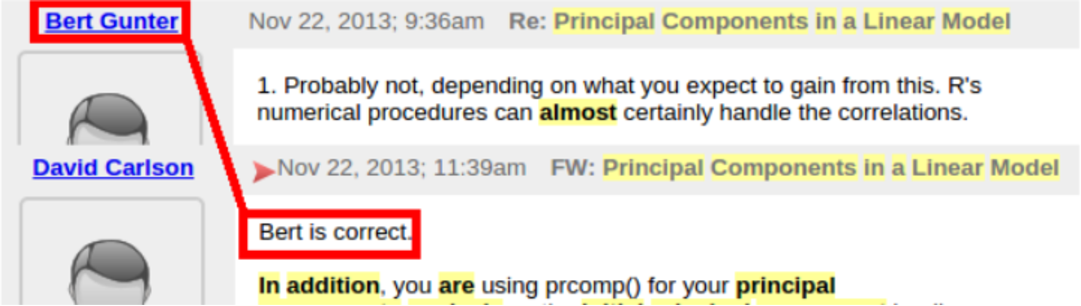
\includegraphics[width=\columnwidth]{Figures/ML-PKimg2}
        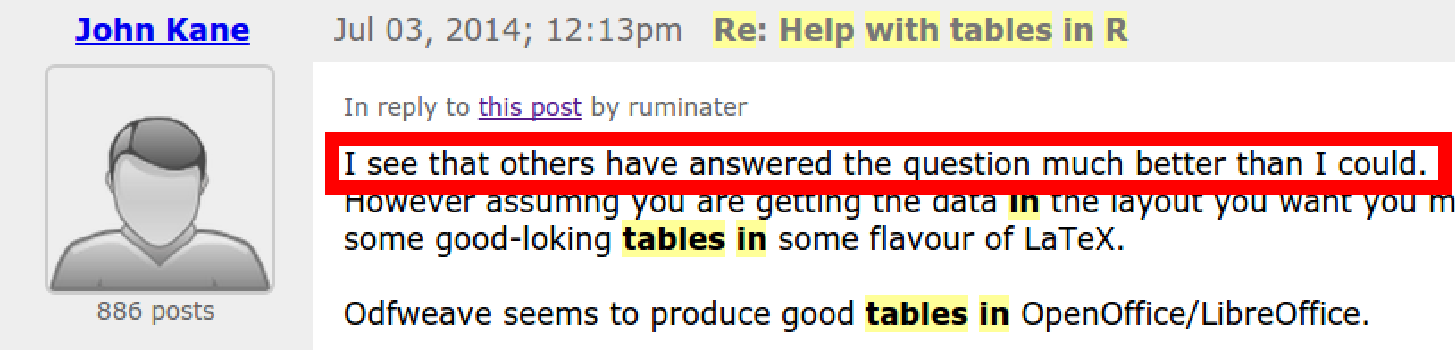
\includegraphics[width=\columnwidth]{Figures/ML-PKimg11}
        \caption[Participatory knowledge on the R-help mailing list.]{Participatory knowledge on the R-help mailing list.}
        \label{fig:ML-PK1}
\vspace{-3mm}
    \end{figure}

    In Stack Overflow, participatory knowledge takes place when:
    \begin{enumerate*}[label=(\arabic*)]
    \item it is possible to infer a link between answers, via either a direct or indirect reference; or
    \item comments complement the answer, or directly cite another author.
    \end{enumerate*}

    In Stack Overflow, participatory knowledge happens in different places, perhaps as a consequence
    of its rich interface.  We observe this type of knowledge construction when a user answers a
    question and directly cites or links to somebody else's  answer in the thread, or when a
    user cites somebody else's question or answer in a comment (a typical case is linking to a previously asked question).
    Figure \ref{fig:SO-PK1} depicts an example of participatory knowledge in Stack Overflow: the
    user has added a comment to help another user when the answer is not sufficient.  In the comment, the user references another author's answer.

    \begin{figure}[!htb]
        \centering
        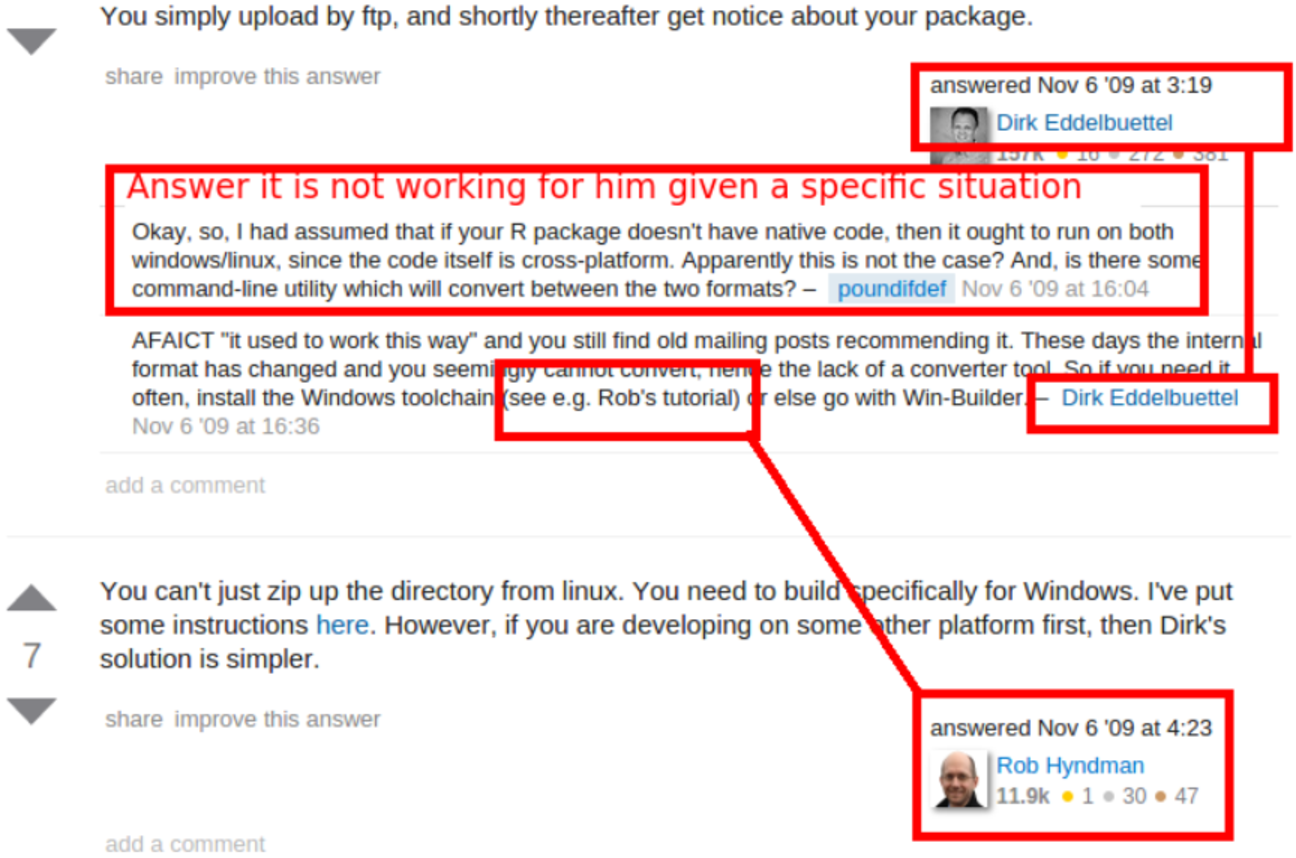
\includegraphics[width=\columnwidth]{Figures/SO-PKimg5}
        \caption{Example of participatory knowledge on Stack Overflow. Users build on the comments and answers of other users.}
        \label{fig:SO-PK1}
\vspace{-3mm}
    \end{figure}

    Crowd knowledge construction is observable when:
    \begin{enumerate*}[label=(\arabic*)]
    \item there is no direct or inferable reference between answers,
    \item answers are a variation of one of the answers on the thread.
    \end{enumerate*}
    Figure \ref{fig:CKC_MLSO} depicts an example of how crowd knowledge construction is visible in Stack Overflow.
    As can be seen from the figure, two of the three answers provided the same solution. 

    \begin{figure} [!htb]
        \centering
        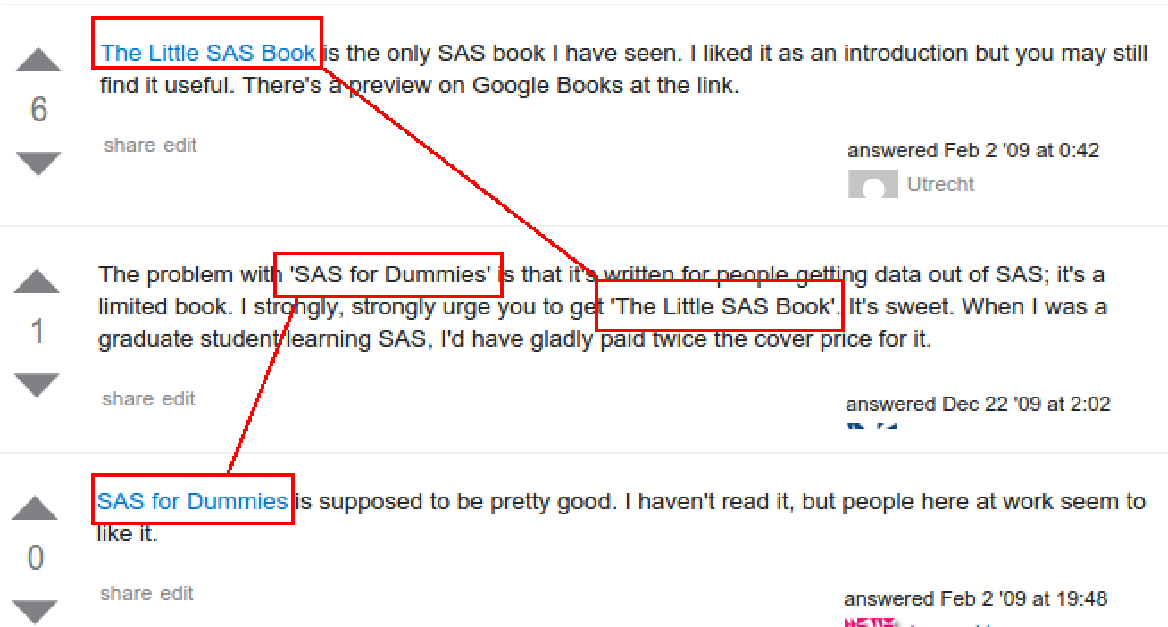
\includegraphics[width=\columnwidth]{Figures/SO-CSimg2}
        \caption{Example of how crowd knowledge construction occurs. The three authors provide similar answers, but they do it independently of each other.}
        \label{fig:CKC_MLSO}
\vspace{-3mm}
    \end{figure}

\subsection{RQ-3. Why do certain users post to both Stack Overflow and the R-help mailing list}

Based on the responses from the survey, we identified that being active on both channels brings benefits to those asking and answering questions:

\begin{description}[itemsep=2pt, topsep=0pt, leftmargin=1em, parsep=0pt]
\item[Find a better answer:] As expected, two channels are better than one. 
  One channel might provide a better answer than the other.
\item[Support follow-up questions:] We found that \RH is often used to have follow-up discussions on
  specific answers to \SO questions. \SO focus is on finding an answer to a question, and does not
  provide an environment to discuss the specifics of an answer (unless it is asked as another question).
In contrast, in \RH, the discussion can continue long after an answer has been found with follow-up questions (not only by the person who asked the original question).  
\item[Speeds up answers:] Users ask the same question on both channels in order to get a faster answer. However, this behaviour s not encouraged by the community as it is deemed impolite\footnote{\href{https://goo.gl/p9vVaj}{https://goo.gl/p9vVaj}}.
% `... it's impolite to cross post across several lists (i.e. stackoverflow and R-help)''
\end{description}

In contrast, some users also stated their preference of one channel over the other. We summarize their responses below:
 

\subsubsection{\SO}

Users preferred \SO for five main reasons:
a) being able to gain peer recognition (the advantage of gaining points---and visibility---is a major draw towards SO);
b) its rich and user friendly interface;
c) answers are straight to the point;
d) questions are usually answered faster in \SO than \RH; and e) it is easy to search for previous questions and answers.

The main drawbacks of using Stack Overflow include: a) an abundance
    of related questions; b) certain level of experience is required to understand some of the answers, and c) \SO strict rules that only allow questions and their answers (\SO does not allow discussions nor questions about opinions).


\subsubsection{\RH}
\label{sec:rh}

The benefits of using \RH include: a) the convenience of just handling email;
 b)  following the mailing list provides awareness and increases learning in new topics;
c) the flexibility of \RH regarding the topics that one can discuss;
and d) the participation of highly experienced users.

The main disadvantages of \RH are: a) sometimes aggressive
behaviour arises during discussions; and b) searching the archives is not easy.


%%% Local Variables:
%%% mode: latex
%%% TeX-master: "knowledge-curation.tex"
%%% End:
